\documentclass[12pt,reqno]{article}
\usepackage[usenames]{color}
\usepackage{amssymb}
\usepackage{amsmath}
\usepackage[colorlinks=true,
linkcolor=webgreen,
filecolor=webbrown,
citecolor=webgreen]{hyperref}
\usepackage{color}
\usepackage{pgfplots}

\begin{document}

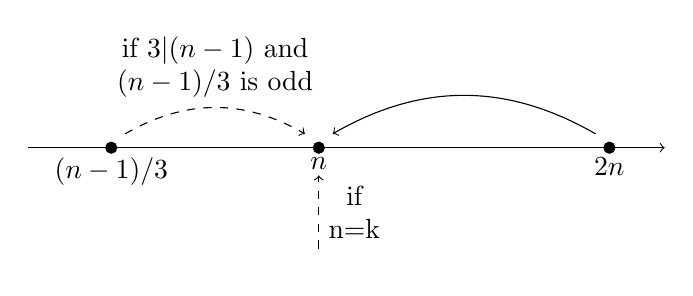
\begin{tikzpicture}
	% n=2, 7 and 14 are scaled by 1.5
	\draw[->] (0,0) -- (23em,0);
	\filldraw[black] (3em,0) circle (2pt) node[below] (f) {$(n-1)/3$};
	\filldraw[black] (10.5em,0) circle (2pt) node[below] (n) {$n$};
	\filldraw[black] (21em,0) circle (2pt) node[below] (b) {$2n$};
	\path[->,dashed] (3.5em,.5em) edge [bend left] node[above,align=center] 
	{if $3|(n-1)$ and\\$(n-1)/3$ is odd} (10em,.5em);
	\path[->] (20.5em,.5em) edge [bend right] node[above] {} (11em,.5em);
	\node at (10.5em, -4em) (s) {};
	\draw[->,dashed] (s) -- node[right,align=center] {if\\n=k} (10.5em,-1em);
	\end{tikzpicture}

\end{document}